\chapter{Casi d'uso}\label{sec:casi}
\section{Introduzione}
In questa sezione del documento vengono riportati tutti i casi d'uso relativi al prodotto del progetto.\\
Ogni caso d'uso sarà identificato da un codice alfanumerico, composto dall'acronimo "UC" di \ccgloss{use case} e seguito da dei numeri. Per ottenere una gerarchizzazione ad albero dei casi d'uso, con cui segnalare un sotto caso d'uso di un altro, i numeri saranno seguiti da uno o più punti, con cui sarà facile identificare il sotto caso d'uso rispetto al padre.\\
Ogni use case sarà inoltre corredato dalle informazioni riguardanti descrizione generale, \ccgloss{attore} principale, pre condizioni, post condizioni e scenario, oltre ad attori secondari, generalizzazioni ed estensioni qualora presenti.

\section{Attori}
A seguito della richiesta esplicita da parte del proponente di non implementare alcun meccanismo di autenticazione, non vengono distinti nell'analisi dei casi d'uso utenti autenticati o meno, né utenti \ccgloss{amministratori}.\\
Per questo motivo, l'unico attore principale di tutti i casi d'uso sarà un utente generico, definito "user" negli \ccgloss{UML} dei casi d'uso.\\
L'attore secondario, definito con l'acronimo \ccgloss{LLM}, identifica il modello large language che è alla base del funzionamento del chatbot e delle funzionalità che permettono l'interazione dell'utente con esso. Il modello è identificato come attore secondario, e non come parte del sistema stesso, in quanto non sarà allenato dal sistema né il sistema avrà alcun potere su di esso.

\begin{figure}[H]
    \centering
    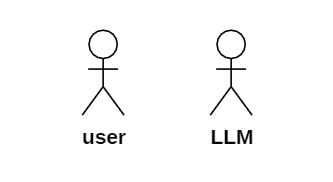
\includegraphics[width=0.4\linewidth]{Attori.PNG}
    \caption{Attori}
    \label{fig:attori}
\end{figure}

\newpage

\section{Elenco dei casi d'uso}

\subsection{UC-1 Visualizza lista LLM}
\begin{description}
    \item[Descrizione:] L’utente vuole visualizzare la lista dei Large Language Model con cui poter utilizzare il sistema.
    \item[Attore primario:] Utente generico.
    \item[Pre condizioni:] Il sistema presenta la lista di tutti i LLM supportati.
    \item[Post condizioni:] Il sistema mostra l’intera lista di tutti i LLM supportati.
    \item[Scenario:] 
    \begin{enumerate}
        \item[]
        \item L’utente visualizza la lista di tutti i LLM utilizzabili per le operazioni del sistema.
    \end{enumerate}
\end{description}

\begin{figure}[H]
    \centering
    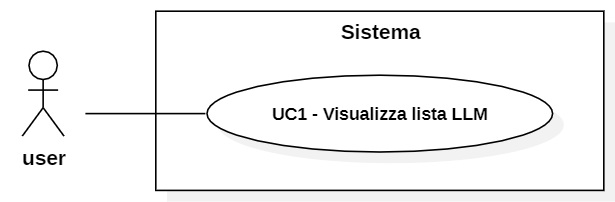
\includegraphics[width=0.8\linewidth]{UC1.PNG}
    \caption{Diagramma UML del caso d'uso UC-1}
    \label{fig:UC1}
\end{figure}

\subsection{UC-2 Seleziona LLM}
\begin{description}
    \item[Descrizione:] L’utente vuole selezionare il LLM da utilizzare nelle operazioni del sistema.
    \item[Attore primario:] Utente generico.
    \item[Pre condizioni:] Il sistema mostra la lista di tutti i LLM supportati.
    \item[Post condizioni:] Il sistema varia il proprio LLM di funzionamento dopo la modifica dell'utente.
    \item[Scenario:] 
    \begin{enumerate}
        \item[]
        \item L’utente visualizza la lista di tutti i LLM utilizzabili per le operazioni del sistema (\textbf{UC-1}).
        \item L'utente seleziona il LLM che il sistema deve utilizzare nelle proprie funzionalità.
    \end{enumerate}
    
\end{description}

\begin{figure}[H]
    \centering
    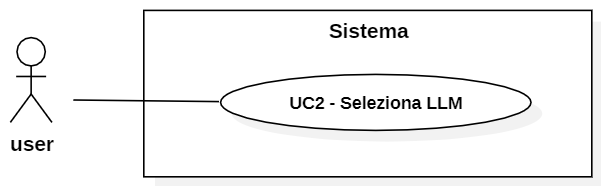
\includegraphics[width=0.8\linewidth]{UC2.PNG}
    \caption{Diagramma UML del caso d'uso UC-2}
    \label{fig:UC2}
\end{figure}

\subsection{UC-3 Visualizza lista documenti}
\begin{description}
    \item[Descrizione:] L’utente vuole visualizzare la lista dei documenti presenti nel sistema.
    \item[Attore primario:] Utente generico.
    \item[Pre condizioni:] Il sistema mostra l’interfaccia di gestione documenti.
    \item[Post condizioni:] Il sistema mostra l’intera lista di documenti.
    \item[Scenario:] 
    \begin{enumerate}
        \item[]
        \item L’utente visualizza la lista di tutti documenti.
    \end{enumerate}
\end{description}

\begin{figure}[H]
    \centering
    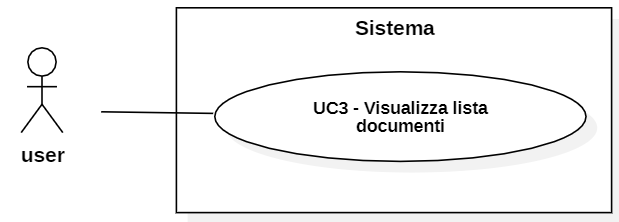
\includegraphics[width=0.8\linewidth]{UC3.PNG}
    \caption{Diagramma UML del caso d'uso UC-3}
    \label{fig:UC3}
\end{figure}

\subsection{UC-4 Visualizza singolo documento}
\begin{description}
    \item[Descrizione:] L'utente vuole visualizzare un particolare documento presente nel sistema.
    \item[Attore primario:] Utente generico.
    \item[Pre condizioni:] Il sistema mostra l’intera lista di documenti.
    \item[Post condizioni:] Il sistema mostra il documento di interesse.
    \item[Scenario:]
    \begin{enumerate}
        \item[]
        \item L’utente visualizza la lista di tutti documenti (\textbf{UC-3}).
        \item L'utente visualizza il singolo documento.
    \end{enumerate} 
\end{description}

\begin{figure}[H]
    \centering
    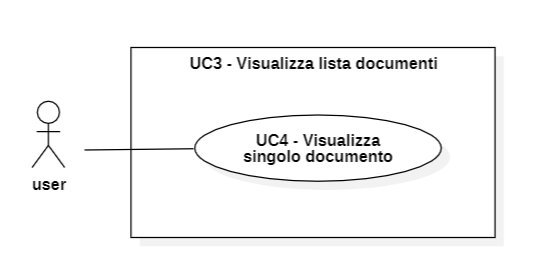
\includegraphics[width=0.8\linewidth]{UC4.PNG}
    \caption{Diagramma UML dei casi d'uso UC-4}
    \label{fig:UC4}
\end{figure}

\subsection{UC-4.1 Visualizza nome del documento}
\begin{description}
    \item[Descrizione:] L'utente vuole visualizzare il nome del documento di interesse.
    \item[Attore primario:] Utente generico.
    \item[Pre condizioni:] Il sistema mostra l’intera lista di documenti.
    \item[Post condizioni:] Il sistema mostra il nome del documento selezionato.
    \item[Scenario:]
    \begin{enumerate}
        \item[]
        \item L’utente visualizza la lista di tutti documenti (\textbf{UC-3}).
        \item L'utente visualizza il singolo documento (\textbf{UC-4}).
        \item L'utente visualizza il nome del documento.
    \end{enumerate} 
\end{description}

\subsection{UC-4.2 Visualizza data di inserimento del documento}
\begin{description}
    \item[Descrizione:] L'utente vuole visualizzare la data di inserimento del documento di interesse.
    \item[Attore primario:] Utente generico.
    \item[Pre condizioni:] Il sistema mostra l’intera lista di documenti.
    \item[Post condizioni:] Il sistema mostra la data di inserimento del documento selezionato.
    \item[Scenario:] 
    \begin{enumerate}
        \item[]
        \item L’utente visualizza la lista di tutti documenti (\textbf{UC-3}).
        \item L'utente visualizza il singolo documento (\textbf{UC-4}).
        \item L'utente visualizza la data di inserimento del documento voluto.
    \end{enumerate}
\end{description}

\subsection{UC-4.3 Visualizza tag del documento}
\begin{description}
    \item[Descrizione:] L'utente vuole visualizzare i tag applicati al documento di interesse.
    \item[Attore primario:] Utente generico.
    \item[Pre condizioni:] Il sistema mostra l’intera lista di documenti.
    \item[Post condizioni:] Il sistema mostra i tag del documento selezionato.
    \item[Scenario:]
    \begin{enumerate}
        \item[]
        \item L’utente visualizza la lista di tutti documenti (\textbf{UC-3}).
        \item L'utente visualizza il singolo documento (\textbf{UC-4}).
        \item L'utente visualizza i tag applicati al documento voluto.
    \end{enumerate}
\end{description}

\subsection{UC-4.4 Visualizza contenuto del documento}
\begin{description}
    \item[Descrizione:] L'utente vuole visualizzare il documento di interesse.
    \item[Attore primario:] Utente generico.
    \item[Pre condizioni:] Il sistema mostra l’intera lista di documenti.
    \item[Post condizioni:] Il sistema mostra il contenuto del documento selezionato.
    \newpage
    \item[Scenario:]
    \begin{enumerate}
        \item[]
        \item L’utente visualizza la lista di tutti documenti (\textbf{UC-3}).
        \item L'utente visualizza il singolo documento (\textbf{UC-4}).
        \item L'utente visualizza il contenuto del documento voluto.
    \end{enumerate}
\end{description}

\subsection{UC-4.5 Visualizza stato del documento}
\begin{description}
    \item[Descrizione:] L'utente vuole visualizzare lo stato del documento di interesse, per sapere se è bloccato o sbloccato.
    \item[Attore primario:] Utente generico.
    \item[Pre condizioni:] Il sistema mostra l’intera lista di documenti.
    \item[Post condizioni:] Il sistema mostra lo stato del documento selezionato.
    \item[Scenario:]
    \begin{enumerate}
        \item[]
        \item L’utente visualizza la lista di tutti documenti (\textbf{UC-3}).
        \item L'utente visualizza il singolo documento (\textbf{UC-4}).
        \item L'utente visualizza lo stato del documento voluto.
    \end{enumerate}
\end{description}

\subsection{UC-4.6 Visualizza dimensione del documento}
\begin{description}
    \item[Descrizione:] L'utente vuole visualizzare la dimensione del documento di interesse.
    \item[Attore primario:] Utente generico.
    \item[Pre condizioni:] Il sistema mostra l’intera lista di documenti.
    \item[Post condizioni:] Il sistema mostra la dimensione del documento selezionato.
    \item[Scenario:]
    \begin{enumerate}
        \item[]
        \item L’utente visualizza la lista di tutti documenti (\textbf{UC-3}).
        \item L'utente visualizza il singolo documento (\textbf{UC-4}).
        \item L'utente visualizza la dimensione del documento voluto.
    \end{enumerate}
\end{description}

\begin{figure}[H]
    \centering
    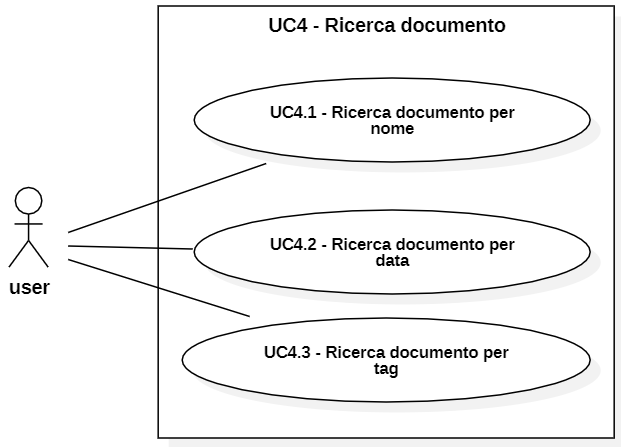
\includegraphics[width=0.8\linewidth]{UC4.1.PNG}
    \caption{Diagramma UML dei casi d'uso UC-4.1, UC-4.2, UC-4.3, UC-4.4, UC-4.5 e UC-4.6}
    \label{fig:UC4.1}
\end{figure}

\subsection{UC-5 Ricerca documento}
\begin{description}
    \item[Descrizione:] L’utente vuole poter ricercare un documento per nome, tag e/o data di inserimento.
    \item[Attore primario:] Utente generico.
    \item[Pre condizioni:] Il sistema mostra l’intera lista di documenti.
    \item[Post condizioni:] Il sistema mostra la lista di documenti che soddisfano la ricerca.
    \item[Scenario:]
    \begin{enumerate}
        \item[]
        \item L’utente seleziona la barra di ricerca per cercare un documento.
    \end{enumerate}
\end{description}

\begin{figure}[H]
    \centering
    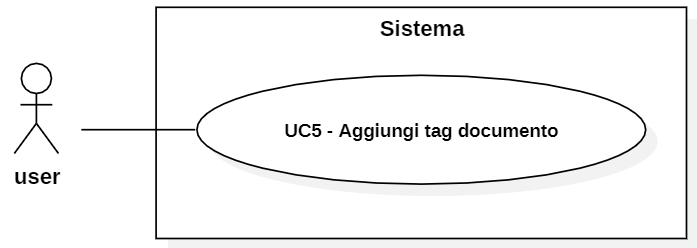
\includegraphics[width=0.8\linewidth]{UC5.PNG}
    \caption{Diagramma UML del caso d'uso UC-5}
    \label{fig:UC5}
\end{figure}

\subsection{UC-5.1 Ricerca documento per nome}
\begin{description}
    \item[Descrizione:] L’utente vuole poter ricercare un documento per nome.
    \item[Attore primario:] Utente generico.
    \item[Pre condizioni:] Il sistema mostra l’intera lista di documenti.
    \item[Post condizioni:] Il sistema mostra la lista di documenti che contengono il nome inserito.
    \item[Scenario:] 
    \begin{enumerate}
        \item[]
        \item L’utente seleziona la barra di ricerca per cercare un documento (\textbf{UC-4}).
        \item L’utente inserisce il nome del file da trovare e invia la ricerca.
    \end{enumerate}
\end{description}

\subsection{UC-5.2 Ricerca documento per data}
\begin{description}
    \item[Descrizione:] L’utente vuole poter ricercare un documento per data di inserimento.
    \item[Attore primario:] Utente generico.
    \item[Pre condizioni:] Il sistema mostra l’intera lista di documenti.
    \item[Post condizioni:] Il sistema mostra la lista di documenti che sono stati inseriti dopo una certa data.
    \item[Scenario:] 
    \begin{enumerate}
        \item[]
        \item L’utente seleziona la barra di ricerca per cercare un documento (\textbf{UC-4}).
        \item L’utente inserisce la data di caricamento del file e avvia la ricerca.
    \end{enumerate}
\end{description}

\subsection{UC-5.3 Ricerca documento per tag}
\begin{description}
    \item[Descrizione:] L’utente vuole poter ricercare un documento per i tag che gli sono stati applicati.
    \item[Attore primario:] Utente generico.
    \item[Pre condizioni:] Il sistema mostra l’intera lista di documenti.
    \item[Post condizioni:] Il sistema mostra la lista di documenti che hanno quel tag.
    \item[Scenario:] 
    \begin{enumerate}
        \item[]
        \item L’utente seleziona la barra di ricerca per cercare un documento (\textbf{UC-4}).
        \item L’utente inserisce il tag che deve aver associato il documento e avvia la ricerca.
    \end{enumerate}
\end{description}

\begin{figure}[H]
    \centering
    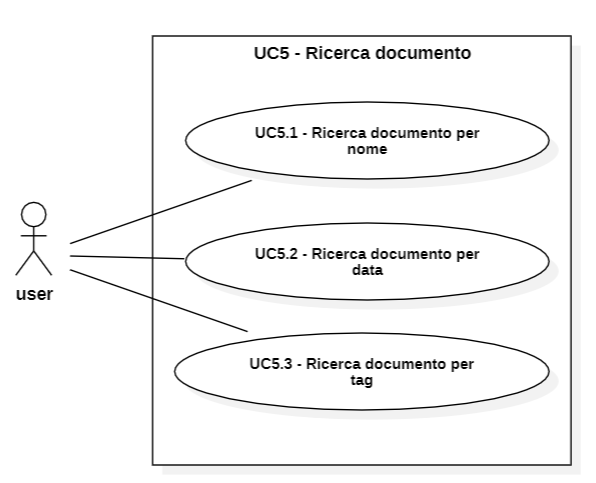
\includegraphics[width=0.8\linewidth]{UC5.1.png}
    \caption{Diagramma UML dei casi d'uso UC-5.1, UC-5.2 e UC-5.3}
    \label{fig:UC5.1-2-3}
\end{figure}

\subsection{UC-6 Aggiungi tag al documento}
\begin{description}
    \item[Descrizione:] L’utente vuole poter aggiungere un tag ad uno dei documenti presenti a sistema.
    \item[Attore primario:] Utente generico.
    \item[Pre condizioni:] Il sistema presenta il tag di interesse dell'utente, che vuole applicare ad un documento che ancora non lo ha.
    \item[Post condizioni:] Il documento ha il nuovo tag selezionato dall’utente.
    \item[Scenario:]
    \begin{enumerate}
        \item[]
        \item L’utente visualizza la lista di tutti documenti (\textbf{UC-3}).
        \item L'utente visualizza il singolo documento (\textbf{UC-4}).
        \item L’utente visualizza la lista di tutti i tag possibili.
        \item L’utente seleziona il tag da aggiungere.
    \end{enumerate}
\end{description}

\begin{figure}[H]
    \centering
    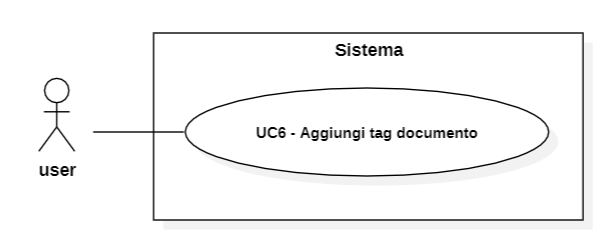
\includegraphics[width=0.8\linewidth]{UC6.png}
    \caption{Diagramma UML del caso d'uso UC-6}
    \label{fig:UC6}
\end{figure}

\subsection{UC-7 Rimuovi tag dal documento}
\begin{description}
    \item[Descrizione:] L’utente vuole poter rimuovere un tag da un documento.
    \item[Attore primario:] Utente generico.
    \item[Pre condizioni:] Il documento ha associato il tag non più voluto dall’utente.
    \item[Post condizioni:] Il documento non ha più associato il tag non voluto dall’utente.
    \item[Scenario:]
    \begin{enumerate}
        \item[]
        \item L’utente visualizza la lista di tutti documenti (\textbf{UC-3}).
        \item L'utente visualizza il singolo documento (\textbf{UC-4}).
        \item L’utente visualizza la lista dei tag associati a quel documento.
        \item L’utente seleziona il tag da rimuovere.
    \end{enumerate}
\end{description}

\begin{figure}[H]
    \centering
    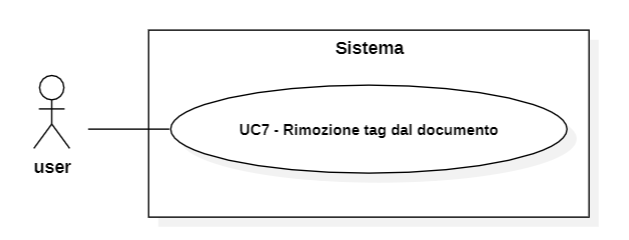
\includegraphics[width=0.8\linewidth]{UC7.png}
    \caption{Diagramma UML del caso d'uso UC-7}
    \label{fig:UC7}
\end{figure}

\subsection{UC-8 Creazione nuovo tag}
\begin{description}
    \item[Descrizione:] L’utente vuole poter creare un tag da poter associare ad un documento.
    \item[Attore primario:] Utente generico.
    \item[Pre condizioni:] Il sistema non presenta il nuovo tag voluto dall’utente.
    \item[Post condizioni:] Il sistema presenta il tag voluto dall’utente.
    \item[Scenario:]
    \begin{enumerate}
        \item[]
        \item L’utente visualizza la lista di tutti i tag (\textbf{UC-9}).
        \item L'utente aggiunge un tag alla lista.
    \end{enumerate}
\end{description}

\begin{figure}[H]
    \centering
    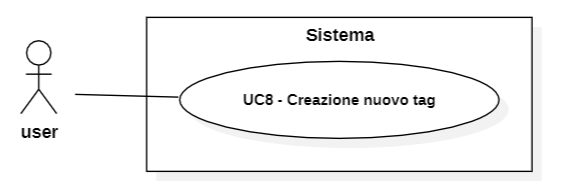
\includegraphics[width=0.8\linewidth]{UC8.png} 
    \caption{Diagramma UML del caso d'uso UC-8}
    \label{fig:UC8}
\end{figure}

\subsection{UC-8.1 Aggiungi nome del tag}
\begin{description}
    \item[Descrizione:] L’utente vuole poter aggiungere un nome nella creazione del tag.
    \item[Attore primario:] Utente generico.
    \item[Pre condizioni:] Il sistema non conosce il nome  il tag voluto dall’utente e il nome associato.
    \item[Post condizioni:] Il sistema conosce il nome del tag voluto dall’utente.
    \item[Scenario:]
    \begin{enumerate}
        \item[]
        \item L’utente visualizza la lista di tutti i tag (\textbf{UC-9}).
        \item L'utente aggiunge un tag alla lista (\textbf{UC-8}).
        \item L'utente inserisce il nome del nuovo tag creato.
    \end{enumerate}
\end{description}

\subsection{UC-8.2 Aggiungi colore del tag}
\begin{description}
    \item[Descrizione:] L’utente vuole poter aggiungere un colore nella creazione del tag.
    \item[Attore primario:] Utente generico.
    \item[Pre condizioni:] Il sistema non conosce il colore il tag voluto dall’utente.
    \item[Post condizioni:] Il sistema conosce il tag voluto dall’utente.
    \item[Scenario:]
    \begin{enumerate}
        \item[]
        \item L’utente visualizza la lista di tutti i tag (\textbf{UC-9}).
        \item L'utente aggiunge un tag alla lista (\textbf{UC-8}).
        \item L'utente inserisce il colore del nuovo tag creato.
    \end{enumerate}
\end{description}

\subsection{UC-8.3 Aggiungi descrizione del tag}
\begin{description}
    \item[Descrizione:] L’utente vuole poter aggiungere una descrizione opzionale nella creazione del tag.
    \item[Attore primario:] Utente generico.
    \item[Pre condizioni:] Il sistema non conosce la descrizione  del tag voluto dall’utente.
    \item[Post condizioni:] Il sistema conosce la descrizione del tag voluto dall’utente.
    \item[Scenario:]
    \begin{enumerate}
        \item[]
        \item L’utente visualizza la lista di tutti i tag (\textbf{UC-9}).
        \item L'utente aggiunge un tag alla lista (\textbf{UC-8}).
        \item L'utente inserisce la descrizione del nuovo tag creato.
    \end{enumerate}
\end{description}
\begin{figure}[H]
    \centering
    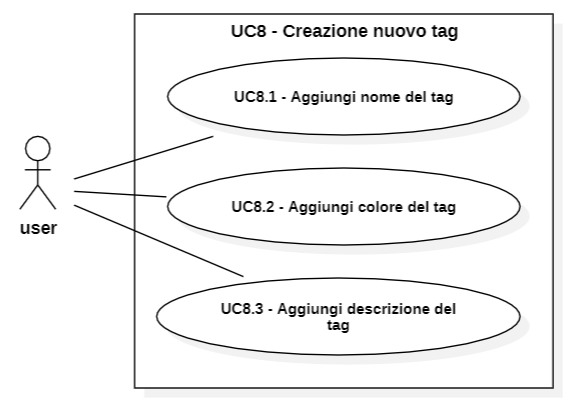
\includegraphics[width=0.8\linewidth]{UC8.1.png} 
    \caption{Diagramma UML dei casi d'uso UC-8.1, UC-8.2 e UC-8.3}
    \label{fig:UC8.1-2-3}
\end{figure}

\subsection{UC-9 Visualizza lista tag}
\begin{description}
    \item[Descrizione:] L’utente vuole poter visualizzare la lista di tutti i tag creati.
    \item[Attore primario:] Utente generico.
    \item[Pre condizioni:] Il sistema mostra l'interfaccia di gestione dei documenti.
    \item[Post condizioni:] Il sistema mostra la lista dei tag creati.
    \item[Scenario:]
    \begin{enumerate}
        \item[]
        \item L’utente visualizza la lista di tutti i tag presenti nel sistema.
    \end{enumerate}
\end{description}
\begin{figure}[H]
    \centering
    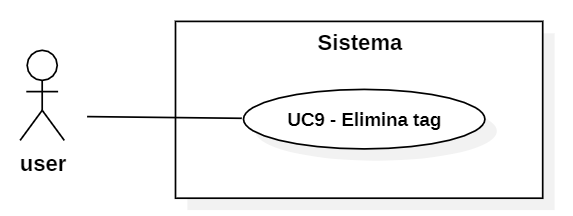
\includegraphics[width=0.8\linewidth]{UC9.PNG}
    \caption{Diagramma UML del caso d'uso UC-9}
    \label{fig:UC9}
\end{figure}

\subsection{UC-10 Visualizza singolo tag}
\begin{description}
    \item[Descrizione:] L’utente vuole poter visualizzare uno dei tag creati.
    \item[Attore primario:] Utente generico.
    \item[Pre condizioni:] Il sistema mostra la lista dei tag creati.
    \item[Post condizioni:] Il sistema mostra il tag di interesse.
    \item[Scenario:]
    \begin{enumerate}
        \item[]
        \item L’utente visualizza la lista di tutti i tag (\textbf{UC-9}).
        \item L'utente visualizza un singolo tag.
    \end{enumerate}
\end{description}

\begin{figure}[H]
    \centering
    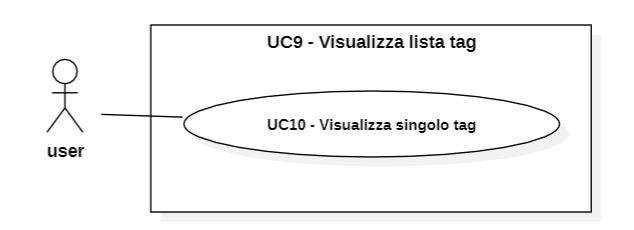
\includegraphics[width=0.8\linewidth]{UC10.png}
    \caption{Diagramma UML del caso d'uso UC-10}
    \label{fig:UC10}
\end{figure}
\subsection{UC-10.1 Visualizza nome del tag}
\begin{description}
    \item[Descrizione:] L’utente vuole poter visualizzare il nome del tag di interesse.
    \item[Attore primario:] Utente generico.
    \item[Pre condizioni:] Il sistema mostra la lista dei tag creati.
    \item[Post condizioni:] Il sistema mostra il nome del tag selezionato.
    \item[Scenario:]
    \begin{enumerate}
        \item[]
        \item L’utente visualizza la lista di tutti i tag (\textbf{UC-9}).
        \item L'utente visualizza un singolo tag (\textbf{UC-10}).
        \item L'utente visualizza il nome del tag.
    \end{enumerate}
\end{description}

\subsection{UC-10.2 Visualizza colore del tag}
\begin{description}
    \item[Descrizione:] L’utente vuole poter visualizzare il colore del tag di interesse.
    \item[Attore primario:] Utente generico.
    \item[Pre condizioni:] Il sistema mostra la lista dei tag creati.
    \item[Post condizioni:] Il sistema mostra il colore del tag selezionato.
    \item[Scenario:] 
    \begin{enumerate}
        \item[]
        \item L’utente visualizza la lista di tutti i tag (\textbf{UC-9}).
        \item L'utente visualizza un singolo tag (\textbf{UC-10}).
        \item L'utente visualizza il colore del tag.
    \end{enumerate}
\end{description}

\subsection{UC-10.3 Visualizza descrizione del tag}
\begin{description}
    \item[Descrizione:] L’utente vuole poter visualizzare la descrizione del tag di interesse.
    \item[Attore primario:] Utente generico.
    \item[Pre condizioni:] Il sistema mostra la lista dei tag creati.
    \item[Post condizioni:] Il sistema mostra la descrizione del tag selezionato.
    \item[Scenario:]
    \begin{enumerate}
        \item[]
        \item L’utente visualizza la lista di tutti i tag (\textbf{UC-9}).
        \item L'utente visualizza un singolo tag (\textbf{UC-10}).
        \item L'utente visualizza la descrizione del tag.
    \end{enumerate}
\end{description}

\begin{figure}[H]
    \centering
    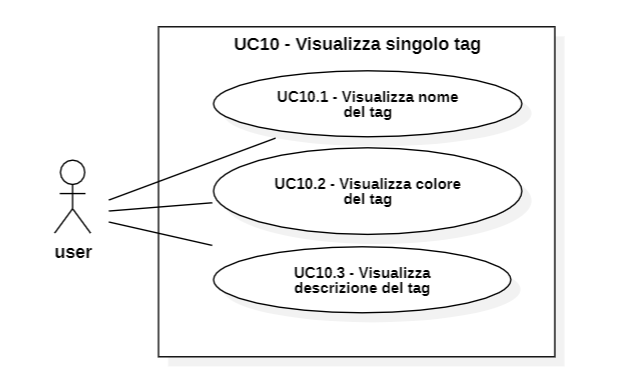
\includegraphics[width=0.8\linewidth]{UC10.1.png}
    \caption{Diagramma UML dei casi d'uso UC-10.1, UC-10.2 e UC-10.3}
    \label{fig:UC10.1}
\end{figure}

\subsection{UC-11 Elimina tag}
\begin{description}
    \item[Descrizione:] L'utente vuole eliminare uno dei tag presenti nel sistema.
    \item[Attore primario:] Utente generico.
    \item[Pre condizioni:] Il sistema presenta il tag non desiderato.
    \item[Post condizioni:] Il sistema non presenta più il tag indesiderato.
    \item[Scenario:]
    \begin{enumerate}
        \item[]
        \item L’utente visualizza la lista di tutti i tag (\textbf{UC-9}).
        \item L'utente visualizza un singolo tag (\textbf{UC-10}).
        \item L'utente elimina il tag visualizzato.
    \end{enumerate}
\end{description}

\begin{figure}[H]
    \centering
    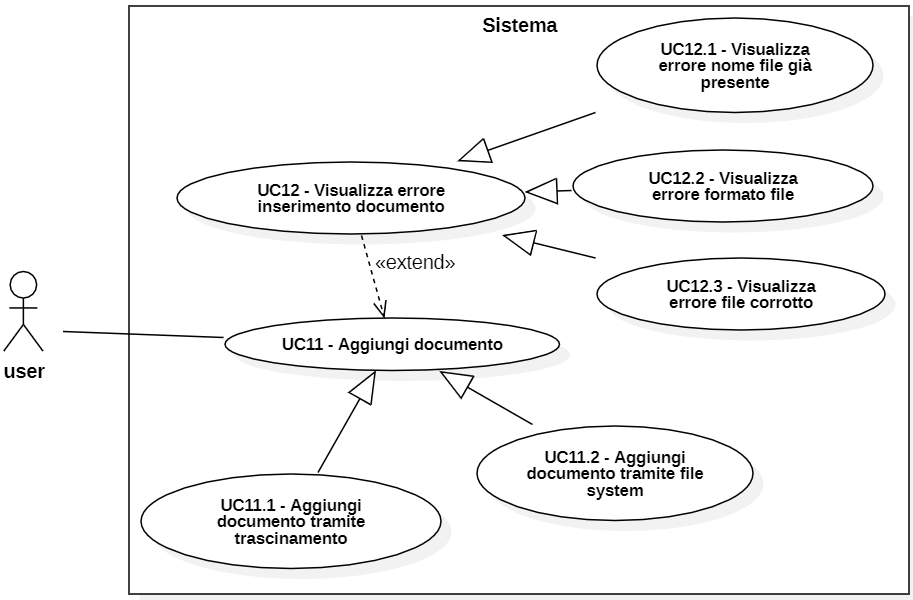
\includegraphics[width=0.8\linewidth]{UC11.PNG} 
    \caption{Diagramma UML del caso d'uso UC-11}
    \label{fig:UC11}
\end{figure}

\subsection{UC-12 Elimina documento}
\begin{description}
    \item[Descrizione:] L'utente vuole eliminare uno dei documenti presenti nel sistema.
    \item[Attore primario:] Utente generico.
    \item[Pre condizioni:] Il sistema presenta il documento non desiderato.
    \item[Post condizioni:] Il sistema non presenta più il documento indesiderato.
    \item[Scenario:]
    \begin{enumerate}
        \item[]
        \item L’utente visualizza la lista di tutti documenti (\textbf{UC-3}).
        \item L'utente visualizza il singolo documento (\textbf{UC-4}).
        \item L'utente elimina il documento d'interesse.
    \end{enumerate} 
\end{description}

\subsection{UC-12.1 Conferma eliminazione documento}
\begin{description}
    \item[Descrizione:] L'utente vuole confermare l'eliminazione di uno dei documenti presenti nel sistema.
    \item[Attore primario:] Utente generico.
    \item[Pre condizioni:] Il sistema presenta il documento non desiderato.
    \item[Post condizioni:] Il sistema non presenta più il documento indesiderato.
    \item[Scenario:] 
    \begin{enumerate}
        \item[]
        \item L’utente visualizza la lista di tutti documenti (\textbf{UC-3}).
        \item L'utente visualizza il singolo documento (\textbf{UC-4}).
        \item L'utente tenta di eliminare il documento d'interesse (\textbf{UC-12}).
        \item L'utente conferma l'eliminazione del documento dal sistema.
    \end{enumerate}
    
\end{description}

\begin{figure}[H]
    \centering
    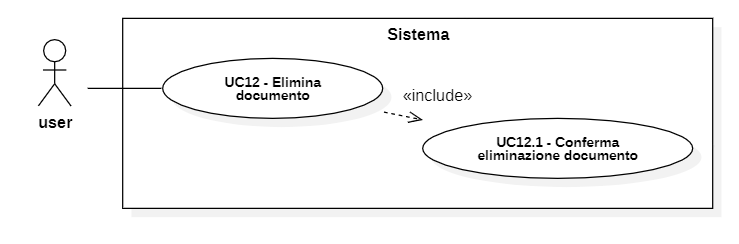
\includegraphics[width=0.8\linewidth]{UC12.PNG}
    \caption{Diagramma UML dei casi d'uso UC-12 e UC-12.1}
    \label{fig:UC12-12.1}
\end{figure}

\subsection{UC-13 Aggiungi documento}
\begin{description}
    \item[Descrizione:] L'utente vuole aggiungere un documento nel sistema.
    \item[Attore primario:] Utente generico.
    \item[Pre condizioni:] Il sistema non presenta il documento di interesse.
    \item[Post condizioni:] Nel sistema è presente un nuovo documento.
    \item[Scenario:]
    \begin{enumerate}
        \item[]
        \item L’utente aggiunge un nuovo documento.
    \end{enumerate}
    \item[Generalizzazioni:] 
    \begin{itemize}
        \item[] 
        \item Aggiungi documento tramite trascinamento (\textbf{UC-13.1});
        \item Aggiungi documento tramite file system (\textbf{UC-13.2}).
    \end{itemize} 
    \item[Scenario alternativo:] Visualizza errore nell'inserimento di un documento (\textbf{UC-14}).
\end{description}

\subsection{UC-13.1 Aggiungi documento tramite trascinamento}
\begin{description}
    \item[Descrizione:] L'utente vuole aggiungere un documento nel sistema tramite trascinamento.
    \item[Attore primario:] Utente generico.
    \item[Pre condizioni:] Il sistema non presenta il documento di interesse.
    \item[Post condizioni:] Nel sistema è presente un nuovo documento.
    \item[Scenario:] 
    \begin{enumerate}
        \item[]
        \item L’utente tenta di aggiungere un nuovo documento (\textbf{UC-13}).
        \item L'utente aggiunge un nuovo documento nel sistema tramite trascinamento.
    \end{enumerate}
\end{description}

\subsection{UC-13.2 Aggiungi documento tramite file system}
\begin{description}
    \item[Descrizione:] L'utente vuole aggiungere un documento nel sistema tramite navigazione del file system.
    \item[Attore primario:] Utente generico.
    \item[Pre condizioni:] Il sistema non presenta il documento di interesse.
    \item[Post condizioni:] Nel sistema è presente un nuovo documento.
    \item[Scenario:]
    \begin{enumerate}
        \item[]
        \item L’utente tenta di aggiungere un nuovo documento (\textbf{UC-13}).
        \item L'utente aggiunge un nuovo documento nel sistema tramite navigazione del file system.
    \end{enumerate}
\end{description}

\subsection{UC-14 Visualizza errore inserimento documento}
\begin{description}
    \item[Descrizione:] L'utente visualizza un messaggio che lo notifica che c'è stato un errore nell'inserimento del documento.
    \item[Attore primario:] Utente generico.
    \item[Pre condizioni:] L'utente tenta di inserire un documento nel sistema.
    \item[Post condizioni:] Il sistema notifica un messaggio di errore e il documento non viene inserito nel sistema.
    \item[Scenario:]
    \begin{enumerate}
        \item[]
        \item L’utente tenta di aggiungere un nuovo documento (\textbf{UC-13}).
        \item L'utente visualizza un messaggio d'errore che  notifica il mancato caricamento del documento. 
    \end{enumerate}
    \item[Generalizzazioni:]
    \begin{itemize}
        \item[] 
        \item Visualizza errore nome file già presente (\textbf{UC-14.1});
        \item Visualizza errore formato file (\textbf{UC-14.2});
        \item Visualizza errore file corrotto (\textbf{UC-14.3}).
    \end{itemize}
\end{description}

\subsection{UC-14.1 Visualizza errore nome file già presente}
\begin{description}
    \item[Descrizione:] L'utente visualizza un messaggio che lo notifica che c'è stato un errore nell'inserimento del documento dovuto al nome del file già in uso.
    \item[Attore primario:] Utente generico.
    \item[Pre condizioni:] L'utente tenta di inserire nel sistema un documento con un nome già in uso.
    \item[Post condizioni:] Il sistema notifica un messaggio di errore e il documento non viene inserito nel sistema.
    \item[Scenario:]
    \begin{enumerate}
        \item[]
        \item L’utente tenta di aggiungere un nuovo documento (\textbf{UC-13}).
        \item Il documento ha lo stesso nome di un altro documento presente a sistema.
        \item L'utente visualizza un messaggio d'errore (\textbf{UC-14}).
        \item Il messaggio notifica la esistenza di un documento con lo stesso nome.
    \end{enumerate}
\end{description}

\subsection{UC-14.2 Visualizza errore formato file}
\begin{description}
    \item[Descrizione:] L'utente visualizza un messaggio che lo notifica che c'è stato un errore nell'inserimento del documento dovuto al formato del file non supportato.
    \item[Attore primario:] Utente generico.
    \item[Pre condizioni:] L'utente tenta di inserire nel sistema un documento con un formato non supportato.
    \item[Post condizioni:] Il sistema notifica un messaggio di errore e il documento non viene inserito nel sistema.
    \item[Scenario:] 
    \begin{enumerate}
        \item[]
        \item L’utente tenta di aggiungere un nuovo documento (\textbf{UC-13}).
        \item Il documento ha un formato non supportato dal sistema.
        \item L'utente visualizza un messaggio d'errore (\textbf{UC-14}).
        \item Il messaggio notifica la non validità del formato del file.
    \end{enumerate}
\end{description}

\subsection{UC-14.3 Visualizza errore file corrotto}
\begin{description}
    \item[Descrizione:] L'utente visualizza un messaggio che lo notifica che c'è stato un errore nell'inserimento del documento dovuto alla corruzione del file.
    \item[Attore primario:] Utente generico.
    \item[Pre condizioni:] L'utente tenta di inserire nel sistema un documento corrotto.
    \item[Post condizioni:] Il sistema notifica un messaggio di errore e il documento non viene inserito nel sistema.
    \item[Scenario:]
    \begin{enumerate}
        \item[]
        \item L’utente tenta di aggiungere un nuovo documento (\textbf{UC-13}).
        \item Il file è corrotto.
        \item L'utente visualizza un messaggio d'errore (\textbf{UC-14}).
        \item Il messaggio notifica la corruzione del file.
    \end{enumerate}
\end{description}

\begin{figure}[H]
    \centering
    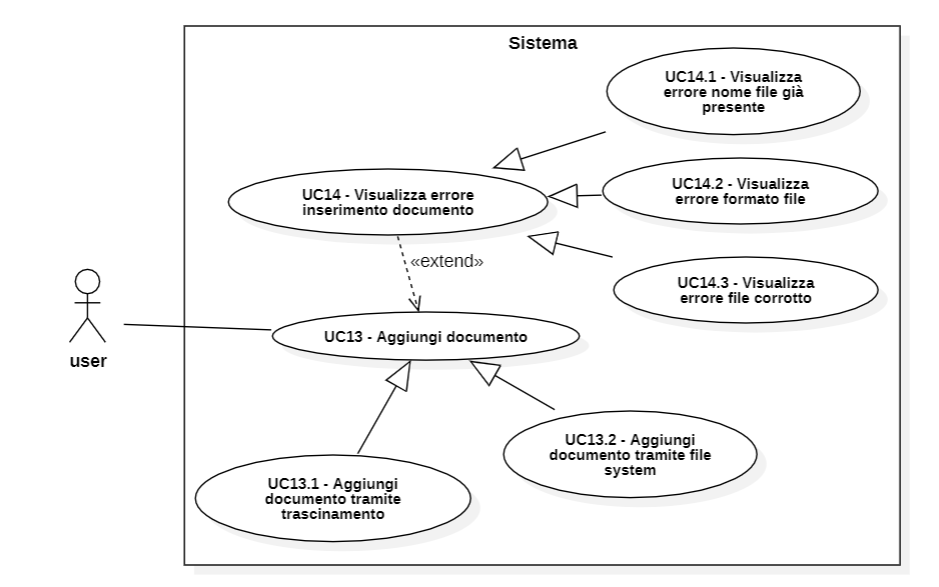
\includegraphics[width=\linewidth]{UC13-14.png}
    \caption{Diagramma UML dei casi d'uso UC-13, UC-13.1, UC-13.2, UC-14, UC-14.1, UC-14.2 e UC-14.3}
    \label{fig:UC13-14}
\end{figure}

\subsection{UC-15 Blocca documento}
\begin{description}
    \item[Descrizione:] L'utente vuole bloccare un documento affinché il chatbot non risponda a domande su di esso, senza doverlo eliminare dal sistema.
    \item[Attore primario:] Utente generico.
    \item[Pre condizioni:] Il sistema presenta un documento di cui può fornire informazioni mediante chatbot.
    \item[Post condizioni:] Il sistema continua a presentare quel documento, ma non è più in grado di fornire informazioni su di esso.
    \item[Scenario:]
    \begin{enumerate}
        \item[]
        \item L’utente visualizza la lista di tutti documenti (\textbf{UC-3}).
        \item L'utente visualizza il singolo documento sbloccato (\textbf{UC-3}).
        \item L'utente blocca il documento che vuole nascondere al sistema.
    \end{enumerate}
\end{description}

\begin{figure}[H]
    \centering
    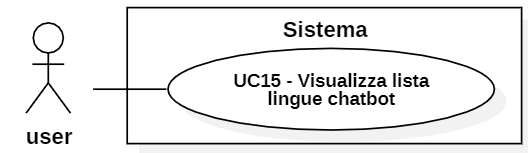
\includegraphics[width=0.8\linewidth]{UC15.PNG}
    \caption{Diagramma UML del caso d'uso UC-15}
    \label{fig:UC15}
\end{figure}

\subsection{UC-16 Sblocca documento}
\begin{description}
    \item[Descrizione:] L'utente vuole sbloccare un documento affinché il chatbot possa nuovamente rispondere a domande su di esso.
    \item[Attore primario:] Utente generico.
    \item[Pre condizioni:] Il sistema presenta un documento di cui non può fornire informazioni mediante chatbot perché bloccato.
    \item[Post condizioni:] Il sistema presenta un documento di cui può fornire informazioni mediante chatbot.
    \newpage
    \item[Scenario:]
    \begin{enumerate}
        \item[]
        \item L’utente visualizza la lista di tutti documenti (\textbf{UC-3}).
        \item L'utente visualizza il singolo documento  (\textbf{UC-4}) che aveva in precedenza bloccato (\textbf{UC-15}).
        \item L'utente sblocca il documento che vuole nascondere al sistema.
    \end{enumerate}
\end{description}

\begin{figure}[H]
    \centering
    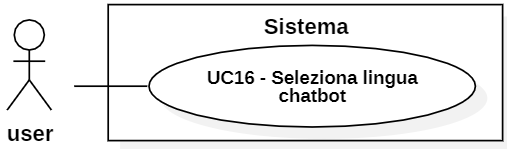
\includegraphics[width=0.8\linewidth]{UC16.PNG}
    \caption{Diagramma UML del caso d'uso UC-16}
    \label{fig:UC16}
\end{figure}

\subsection{UC-17 Visualizza lista lingue chatbot}
\begin{description}
    \item[Descrizione:] L'utente vuole visualizzare la lista delle lingue supportate dal chatbot.
    \item[Attore primario:] Utente generico.
    \item[Pre condizioni:] Il sistema mostra l'interfaccia del chatbot.
    \item[Post condizioni:] Il sistema mostra la lista delle lingue supportate.
    \item[Scenario:]
    \begin{enumerate}
        \item[]
        \item L'utente visualizza la lista delle lingue supportate
    \end{enumerate}
\end{description}

\begin{figure}[H]
    \centering
    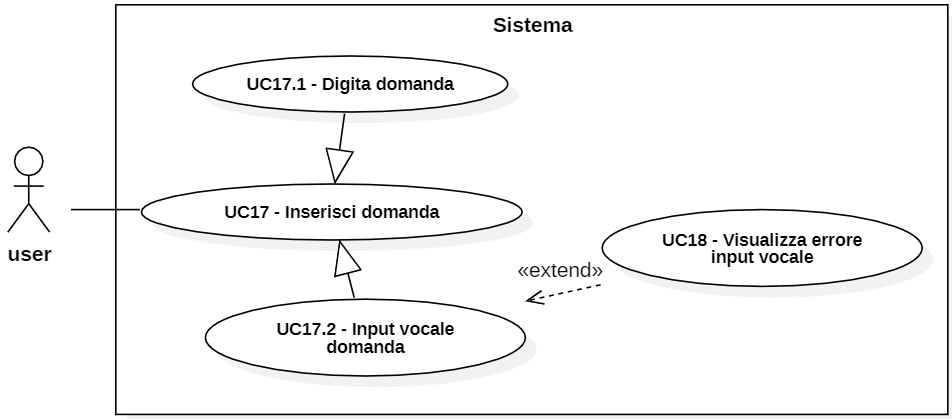
\includegraphics[width=0.8\linewidth]{UC17.PNG}
    \caption{Diagramma UML del caso d'uso UC-17}
    \label{fig:UC17}
\end{figure}

\subsection{UC-18 Seleziona lingua del chatbot}
\begin{description}
    \item[Descrizione:] L'utente vuole selezionare la lingua del sistema.
    \item[Attore primario:] Utente generico.
    \item[Pre condizioni:] Il sistema mostra la lista delle lingue supportate.
    \item[Post condizioni:] Il sistema aggiorna la lingua del chatbot.
    \item[Scenario:]
    \begin{enumerate}
        \item[]
        \item L'utente visualizza la lista delle lingue supportate (\textbf{UC-17})
        \item L’utente seleziona la lingua del chatbot tra quelle supportate.
    \end{enumerate}
\end{description}

\begin{figure}[H]
    \centering
    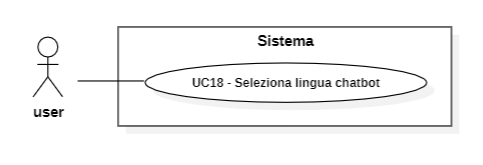
\includegraphics[width=0.8\linewidth]{UC18.PNG}
    \caption{Diagramma UML del caso d'uso UC-18}
    \label{fig:UC18}
\end{figure}

\subsection{UC-19 Inserisci domanda}
\begin{description}
    \item[Descrizione:] L'utente vuole inserire una domanda per il chatbot.
    \item[Attore primario:] Utente generico.
    \item[Pre condizioni:] Il sistema mostra l'interfaccia del chatbot.
    \item[Post condizioni:] La domanda viene inviata al sistema per essere processata.
    \item[Scenario:]
    \begin{enumerate}
        \item[]
        \item L’utente pone una domanda al chatbot.
    \end{enumerate}
    \item[Generalizzazioni:] 
    \begin{itemize}
        \item[] 
        \item Digita domanda (\textbf{UC-19.1});
        \item Input vocale della domanda (\textbf{UC-19.2}) .
    \end{itemize}
\end{description}

\subsection{UC-19.1 Digita domanda}
\begin{description}
    \item[Descrizione:] L'utente vuole digitare la domanda da porgere al chatbot.
    \item[Attore primario:] Utente generico.
    \item[Pre condizioni:] Il sistema mostra l'interfaccia del chatbot dove poter inserire la domanda.
    \item[Post condizioni:] La domanda viene inviata al sistema per essere processata.
    \item[Scenario:]
    \begin{enumerate}
        \item[]
        \item L’utente tenta di porre una domanda al chatbot (\textbf{UC-19}).
        \item L'utente inserisce la domanda da rivolgere al sistema digitandola.
    \end{enumerate}
\end{description}

\subsection{UC-19.2 Input vocale della domanda}
\begin{description}
    \item[Descrizione:] L'utente vuole inserire tramite microfono la domanda da porgere al sistema.
    \item[Attore primario:] Utente generico.
    \item[Pre condizioni:] Il sistema mostra l'interfaccia del chatbot.
    \item[Post condizioni:] La domanda, posta a voce, viene trascritta e inviata al sistema per essere processata.
    \item[Scenario:]
    \begin{enumerate}
        \item[]
        \item L’utente tenta di porre una domanda al chatbot (\textbf{UC-19}).
        \item L'utente inserisce la domanda da rivolgere al chatbot tramite input vocale.
    \end{enumerate}
    \item[Scenario alternativo:] Visualizza errore nell'inserimento della domanda tramite input vocale (\textbf{UC-18}).
\end{description}

\subsection{UC-20 Visualizza errore input vocale}
\begin{description}
    \item[Descrizione:] L'utente visualizza un messaggio che lo informa che non è stato rilevato alcun suono, annullando la trascrizione dell'input vocale.
    \item[Attore primario:] Utente generico.
    \item[Pre condizioni:] L'utente tenta di inserire la domanda tramite input vocale, senza poi produrre alcun suono utile alla trascrizione.
    \item[Post condizioni:] Il sistema non presenta alcuna domanda posta a voce dall'utente e trascritta da inviare al sistema.
    \item[Scenario:] 
    \begin{enumerate}
        \item[]
        \item L’utente vuole porre una domanda al chatbot (\textbf{UC-19}).
        \item L'utente tenta di inserire una domanda da rivolgere al chatbot tramite input vocale (\textbf{UC-19.2}).
        \item Non viene rilevato alcun input vocale.
        \item L'utente visualizza un messaggio di errore, a seguito di un tentativo fallito di inserire tramite input vocale la domanda da porre al sistema.
    \end{enumerate}
\end{description}

\begin{figure}[H]
    \centering
    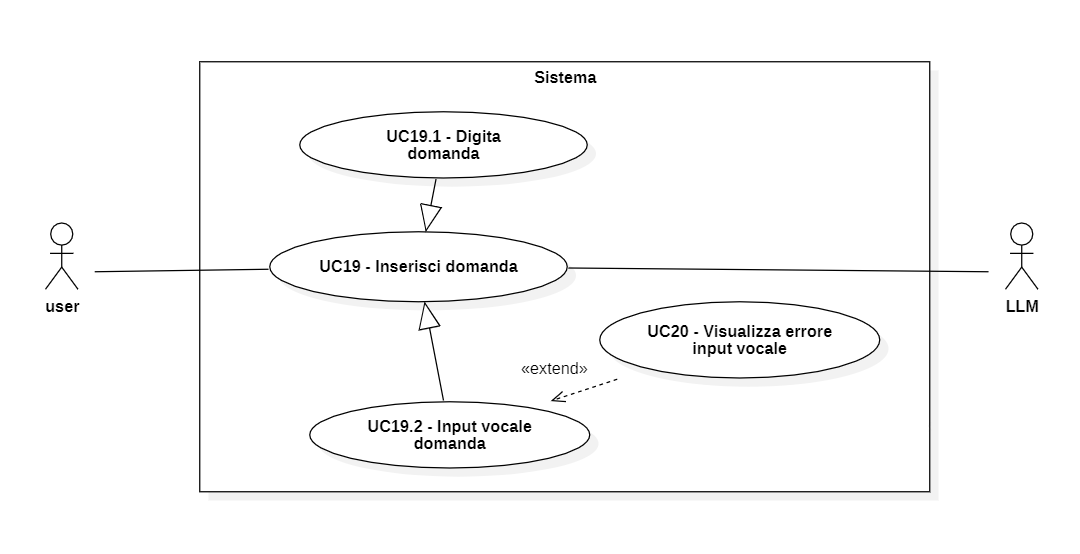
\includegraphics[width=\linewidth]{UC19-20.png}
    \caption{Diagramma UML dei casi d'uso UC-19, UC-19.1, UC-19.2 e 20}
    \label{fig:UC19-20}
\end{figure}

\subsection{UC-21 Visualizza risposta}
\begin{description}
    \item[Descrizione:] L'utente visualizza una risposta dal sistema dopo aver posto una domanda.
    \item[Attore primario:] Utente generico.
    \item[Attore secondario:] Modello LLM. 
    \item[Pre condizioni:] Il sistema ha ricevuto e processato la domanda posta dall'utente.
    \item[Post condizioni:] Il sistema restituisce una risposta all'utente.
    
    \item[Scenario:]
    \begin{enumerate}
        \item[]
        \item L’utente pone una domanda al chatbot (\textbf{UC-19}).
        \item L'utente visualizza la risposta alla domanda posta al sistema.
    \end{enumerate}
    \item[Generalizzazioni:]
    \begin{itemize}
        \item[] 
        \item Visualizza risposta alla domanda (\textbf{UC-21.1});
        \item Visualizza risposta di cortesia (\textbf{UC-21.2}).
    \end{itemize}
    \item[Scenario alternativo:] Visualizza messaggio di errore nella risposta (\textbf{UC-20}).
\end{description}

\subsection{UC-21.1 Visualizza risposta domanda}
\begin{description}
    \item[Descrizione:] L'utente visualizza la risposta alla domanda che ha inviato in precedenza.
    \item[Attore primario:] Utente generico.
    \item[Attore secondario:] Modello LLM. 
    \item[Pre condizioni:] Il sistema ha ricevuto e processato la domanda posta dall'utente, riguardante uno dei documenti inseriti a sistema dall'utente in precedenza.
    \item[Post condizioni:] Il sistema restituisce una risposta della domanda all'utente.
    \item[Scenario:]
    \begin{enumerate}
        \item[]
        \item L’utente inserisce un documento nel sistema (\textbf{UC-11}).
        \item L’utente pone una domanda, pertinente ad uno dei documenti presenti a sistema (\textbf{UC-17}).
        \item L'utente visualizza la risposta alla domanda posta al sistema.
    \end{enumerate}
    \item[Scenario alternativo:] Visualizza messaggio di errore nella risposta (\textbf{UC-22}).
\end{description}

\subsection{UC-21.2 Visualizza risposta di cortesia}
\begin{description}
    \item[Descrizione:] L'utente riceve dal sistema una risposta di cortesia, che lo informa che non può rispondere alla domanda precedentemente posta.
    \item[Attore primario:] Utente generico.
    \item[Attore secondario:] Modello LLM. 
    \item[Pre condizioni:] Il sistema ha ricevuto e processato la domanda posta dall'utente.
    \item[Post condizioni:] Il sistema restituisce una risposta di cortesia all'utente.
    \item[Scenario:]
    \begin{enumerate}
        \item[]
        \item L’utente pone una domanda al chatbot, non pertinente ad alcun documento a sistema (\textbf{UC-19}).
        \item L'utente visualizza la risposta di cortesia alla domanda posta al sistema.
    \end{enumerate}
    \item[Scenario alternativo:] Visualizza messaggio di errore nella risposta (\textbf{UC-20}).
\end{description}

\subsection{UC-22 Visualizza errore risposta}
\begin{description}
    \item[Descrizione:] L'utente visualizza un messaggio dal sistema che lo informa che non è stata prodotta alcuna risposta in tempo utile alla domanda precedentemente posta.
    \item[Attore primario:] Utente generico.
    \item[Pre condizioni:] L'utente pone una domanda al sistema che, dopo essere processata, non produce in tempo alcuna risposta.
    \item[Post condizioni:] Il sistema notifica un messaggio di errore e non restituisce nessuna risposta alla domanda posta.
    \item[Scenario:] 
    \begin{enumerate}
        \item[]
        \item L’utente pone una domanda al chatbot (\textbf{UC-19}).
        \item Il sistema non restituisce in tempo utile una risposta.
        \item L'utente visualizza un errore nella visualizzazione della risposta.
    \end{enumerate}
\end{description}

\begin{figure}[H]
    \centering
    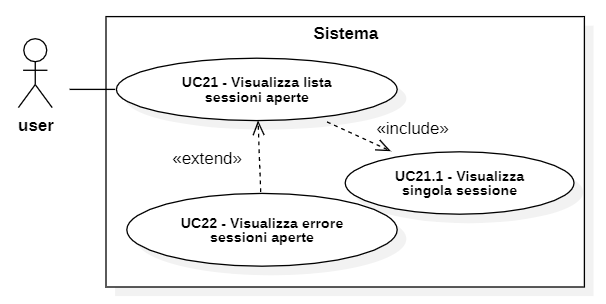
\includegraphics[width=0.77\linewidth]{UC21-22.PNG} 
    \caption{Diagramma UML dei casi d'uso UC-21, UC-21.1, UC-21.2 e UC-22}
    \label{fig:UC21-22}
\end{figure}

\subsection{UC-23 Crea nuova sessione}
\begin{description}
    \item[Descrizione:] L'utente vuole creare una nuova sessione di conversazione col chatbot, che prenderà il nome del primo messaggio inviato.
    \item[Attore primario:] Utente generico.
    \item[Pre condizioni:] Il sistema non presenta la nuova sessione di interesse dell'utente.
    \item[Post condizioni:] Il sistema inizializza una nuova sessione.
    \item[Scenario:] 
    \begin{enumerate}
        \item[]
        \item L'utente crea una nuova sessione di conversazione nel sistema, inviando il primo messaggio (\textbf{UC-19}). 
    \end{enumerate}
\end{description}

\begin{figure}[H]
    \centering
    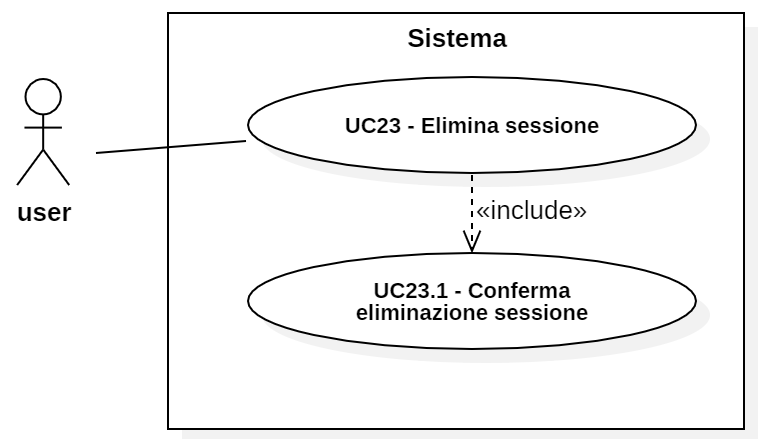
\includegraphics[width=0.8\linewidth]{UC23.PNG} 
    \caption{Diagramma UML del caso d'uso UC-23}
    \label{fig:UC23}
\end{figure}

\subsection{UC-24 Visualizza lista sessioni aperte}
\begin{description}
    \item[Descrizione:] L'utente vuole visualizzare la lista delle sessioni di conversazione col chatbot aperte.
    \item[Attore primario:] Utente generico.
    \item[Pre condizioni:] Il sistema mostra l'interfaccia relativa al chatbot.
    \item[Post condizioni:] Il sistema mostra la lista delle sessioni attive.
    \item[Scenario:]
    \begin{enumerate}
        \item[]
        \item L'utente visualizza la lista delle sessioni attive.
    \end{enumerate}
\end{description}

\begin{figure}[H]
    \centering
    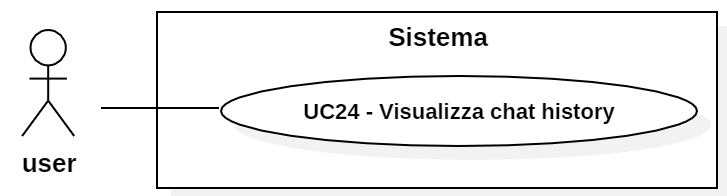
\includegraphics[width=0.8\linewidth]{UC24.PNG}
    \caption{Diagramma UML del caso d'uso UC-24}
    \label{fig:UC24}
\end{figure}

\subsection{UC-24.1 Visualizza singola sessione}
\begin{description}
    \item[Descrizione:] L'utente vuole visualizzare una delle sessioni di conversazione col chatbot.
    \item[Attore primario:] Utente generico.
    \item[Pre condizioni:] Il sistema mostra la lista delle sessioni attive.
    \item[Post condizioni:] Il sistema mostra una particolare sessione attiva, contenente una conversazione tra utente e chatbot.
    \item[Scenario:] 
    \begin{enumerate}
        \item[]
        \item L'utente visualizza la lista delle sessioni attive (\textbf{UC-24}).
        \item L'utente visualizza una delle sessioni attive nel sistema, contenente una conversazione tra utente e chatbot.
    \end{enumerate}
\end{description}

\begin{figure}[H]
    \centering
    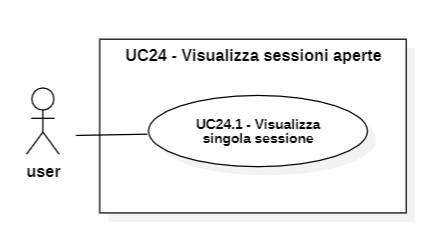
\includegraphics[width=0.8\linewidth]{UC24.1.PNG}
    \caption{Diagramma UML del caso d'uso UC-24.1}
    \label{fig:UC24.1}
\end{figure}

\subsection{UC-24.1.1 Visualizza titolo della singola sessione}
\begin{description}
    \item[Descrizione:] L'utente vuole visualizzare il titolo di una delle sessioni di conversazione col chatbot.
    \item[Attore primario:] Utente generico.
    \item[Pre condizioni:] Il sistema mostra la lista delle sessioni attive.
    \item[Post condizioni:] Il sistema mostra una particolare sessione attiva e con essa il titolo associato.
    \item[Scenario:] 
    \begin{enumerate}
        \item[]
        \item L'utente visualizza la lista delle sessioni attive (\textbf{UC-24}).
        \item L'utente visualizza una delle sessioni attive nel sistema(\textbf{UC-24.1}).
        \item L'utente visualizza il titolo della sessione.
    \end{enumerate}
\end{description}

\begin{figure}[H]
    \centering
    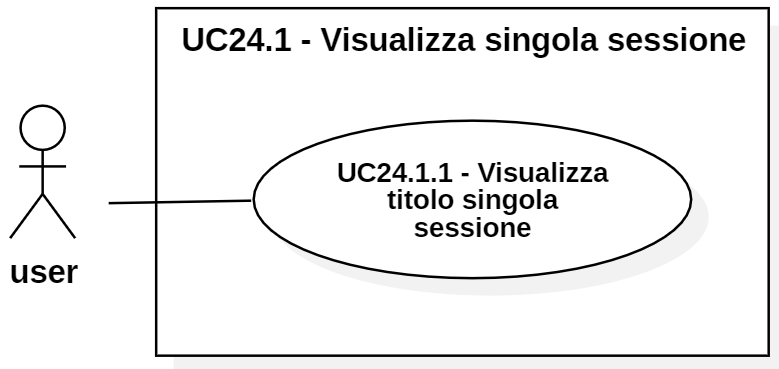
\includegraphics[width=0.8\linewidth]{UC24.1.1.PNG}
    \caption{Diagramma UML del caso d'uso UC-24.1.1}
    \label{fig:UC24.1}
\end{figure}

\subsection{UC-25 Elimina sessioni}
\begin{description}
    \item[Descrizione:] L'utente vuole eliminare tutte le sessioni di conversazione attive nel sistema.
    \item[Attore primario:] Utente generico.
    \item[Pre condizioni:] Il sistema presenta le sessioni, contenenti i messaggi scambiati tra utente e sistema.
    \item[Post condizioni:] Il sistema non presenta più le sessioni eliminate dall'utente, né i messaggi scambiati in essa.
    \item[Scenario:] 
    \begin{enumerate}
        \item[]
        \item L'utente visualizza la lista delle sessioni attive (\textbf{UC-24}).
        \item L'utente elimina dal sistema le sessioni di conversazione con il chatbot.
    \end{enumerate}
\end{description}

\subsection{UC-25.1 Conferma eliminazione sessioni}
\begin{description}
    \item[Descrizione:] L'utente vuole eliminare le sessioni di conversazione attive nel sistema.
    \item[Attore primario:] Utente generico.
    \item[Pre condizioni:] Il sistema presenta le sessione che l'utente tenta di eliminare.
    \item[Post condizioni:] Il sistema non presenta più le sessioni, né i messaggi scambiati in esse.
    \item[Scenario:] 
    \begin{enumerate}
        \item[]
        \item L'utente visualizza la lista delle sessioni attive (\textbf{UC-24}).
        \item L'utente tenta di eliminare dal sistema le sessioni di conversazione con il chatbot (\textbf{UC-25}).
        \item L'utente conferma l'eliminazione delle sessioni di conversazione dal sistema.
    \end{enumerate}
\end{description}

\begin{figure}[H]
    \centering
    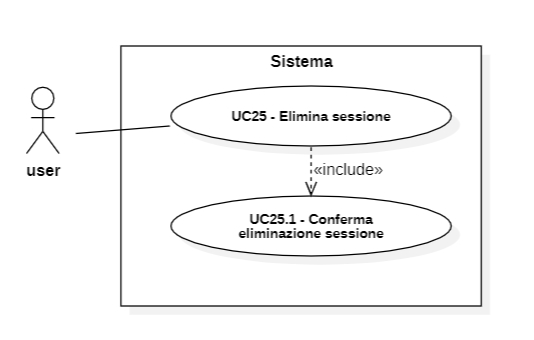
\includegraphics[width=0.8\linewidth]{UC25.png} 
    \caption{Diagramma UML dei casi d'uso UC-25 e UC-25.1}
    \label{fig:UC25}
\end{figure}

\subsection{UC-26 Visualizza \ccgloss{chat history}}
\begin{description}
    \item[Descrizione:] L'utente vuole visualizzare lo scambio di domande e risposte avvenuto in precedenza con il sistema in una sessione.
    \item[Attore primario:] Utente generico.
    \item[Pre condizioni:] Il sistema ha in precedenza ricevuto una o più domande a cui ha fornito risposte.
    \item[Post condizioni:] Il sistema mostra lo storico delle conversazioni dell'utente.
    \item[Scenario:]
    \begin{enumerate}
        \item[]
        \item L'utente visualizza una particolare sessione di conversazione (\textbf{UC-24.1}).
        \item L'utente ha, in precedenza, inviato al sistema delle domande (\textbf{UC-19}), di cui ha ricevuto risposte (\textbf{UC-21}).
        \item L'utente visualizza lo scambio di domande e risposte in una sessione con il sistema.
    \end{enumerate}
    
\end{description} 

\begin{figure}[H]
    \centering
    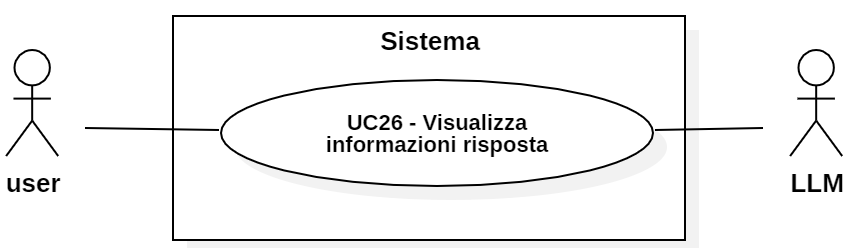
\includegraphics[width=0.9\linewidth]{UC26.PNG}
    \caption{Diagramma UML del caso d'uso UC-26}
    \label{fig:UC26}
\end{figure}

\subsection{UC-26.1 Visualizza singolo messaggio}
\begin{description}
    \item[Descrizione:] L'utente vuole visualizzare il singolo messaggio contenuto nello scambio di domande e risposte, avvenuto in precedenza con il sistema, in una sessione.
    \item[Attore primario:] Utente generico.
    \item[Pre condizioni:] Il sistema mostra la chat history di una sessione.
    \item[Post condizioni:] Il sistema mostra il singolo messaggio di una sessione.
    \item[Scenario:]
    \begin{enumerate}
        \item[]
        \item L'utente visualizza una particolare sessione di conversazione (\textbf{UC-24.1}).
        \item L'utente ha, in precedenza, inviato al sistema delle domande (\textbf{UC-19}), di cui ha ricevuto risposte (\textbf{UC-21}).
        \item L'utente visualizza lo scambio di domande e risposte in una sessione con il sistema (\textbf{UC-26}).
        \item L'utente visualizza un singolo messaggio.
    \end{enumerate}
    
\end{description} 

\begin{figure}[H]
    \centering
    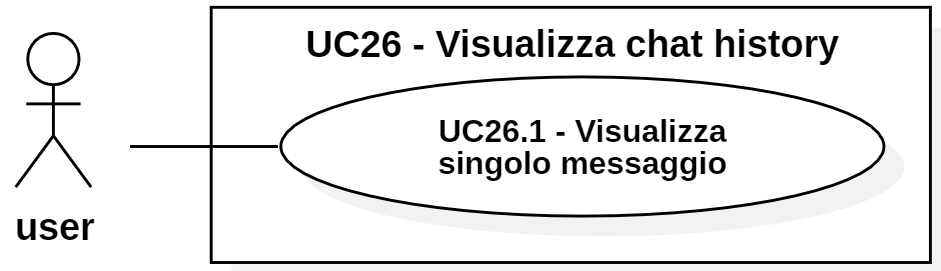
\includegraphics[width=0.9\linewidth]{UC26.1.PNG}
    \caption{Diagramma UML del caso d'uso UC-26.1}
    \label{fig:UC26.1}
\end{figure}

\subsection{UC-27 Elimina singola sessione}
\begin{description}
    \item[Descrizione:] L'utente vuole eliminare una particolare sessione di conversazione dal sistema, e con essa lo scambio di domande e risposte avvenuto in precedenza con il chatbot.
    \item[Attore primario:] Utente generico.
    \item[Pre condizioni:] Il sistema presenta la chat history di una conversazione tenuta in una sessione.
    \item[Post condizioni:] Il sistema non presenta più quella sessione.
    \item[Scenario:]
    \begin{enumerate}
        \item[]
        \item L'utente visualizza una particolare sessione di conversazione (\textbf{UC-24.1}).
        \item L'utente ha, in precedenza, inviato al sistema delle domande (\textbf{UC-19}), di cui ha ricevuto risposte (\textbf{UC-21}).
        \item L'utente visualizza la chat history (\textbf{UC-26}).
        \item L'utente elimina la chat history e la sessione corrente.
    \end{enumerate}
\end{description}

\subsection{UC-27.1 Conferma eliminazione singola sessione}
\begin{description}
    \item[Descrizione:] L'utente vuole confermare l'eliminazione di una particolare sessione di conversazione dal sistema, e con essa lo scambio di domande e risposte avvenuto in precedenza con il chatbot.
    \item[Attore primario:] Utente generico.
    \item[Pre condizioni:] Il sistema presenta la chat history di una conversazione tenuta in una sessione che l'utente ha tentato di eliminare.
    \item[Post condizioni:] Il sistema non presenta più quella sessione.
    \item[Scenario:]
    \begin{enumerate}
        \item[]
        \item L'utente tenta di eliminare la sessione corrente (\textbf{UC-27}).
        \item L'utente conferma l'eliminazione della sessione e della chat history associata dal sistema.
    \end{enumerate}
\end{description}

\begin{figure}[H]
    \centering
    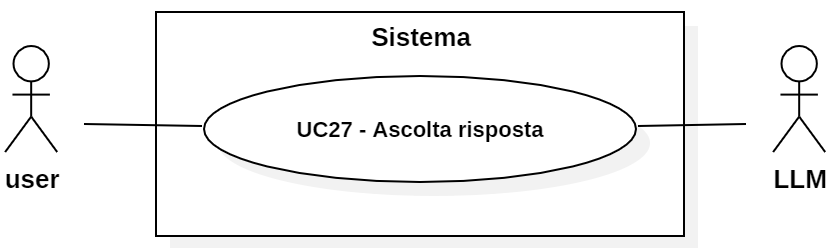
\includegraphics[width=0.8\linewidth]{UC27.PNG} 
    \caption{Diagramma UML dei casi d'uso UC-27 e 27.1}
    \label{fig:UC27}
\end{figure}

\subsection{UC-28 Visualizza fonti risposta}
\begin{description}
    \item[Descrizione:] L'utente vuole visualizzare le informazioni del documento da cui deriva la risposta ricevuta.
    \item[Attore primario:] Utente generico.
    \item[Attore secondario:] Modello LLM.
    \item[Pre condizioni:] Il sistema mostra la risposta ad una domanda dell'utente.
    \item[Post condizioni:] Il sistema mostra le informazioni riguardanti la fonte della risposta.
    \item[Scenario:]
    \begin{enumerate}
        \item[]
        \item L’utente pone una domanda al chatbot (\textbf{UC-19}).
        \item L'utente visualizza la risposta alla domanda posta al sistema (\textbf{UC-21}).
        \item L'utente visualizza le informazioni sul documento fonte della risposta.
    \end{enumerate}
\end{description}

\begin{figure}[H]
    \centering
    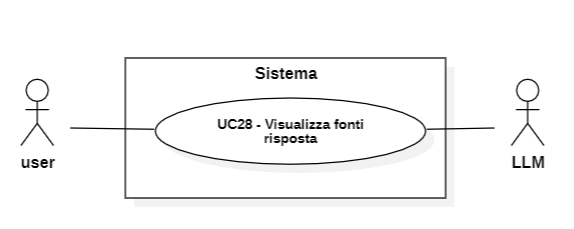
\includegraphics[width=0.9\linewidth]{UC28.PNG}
    \caption{Diagramma UML del caso d'uso UC-28}
    \label{fig:UC28}
\end{figure}

\subsection{UC-28.1 Visualizza nome del documento}
\begin{description}
    \item[Descrizione:] L'utente vuole poter visualizzare il nome del documento relativo alla risposta.
    \item[Attore primario:] Utente generico.
    \item[Attore secondario:] Modello LLM.
    \item[Pre condizioni:] Il sistema non visualizza il nome del documento.
    \item[Post condizioni:] Il sistema visualizza il nome del documento.
    \item[Scenario:] 
    \begin{enumerate}
        \item[]
        \item L’utente pone una domanda al chatbot (\textbf{UC-19}).
        \item L'utente visualizza la risposta alla domanda posta al sistema (\textbf{UC-21}).
        \item L'utente visualizza le informazioni sul documento fonte della risposta (\textbf{UC-28}).
        \item L'utente visualizza il nome del documento.
    \end{enumerate}
\end{description}

\subsection{UC-28.2 Visualizza pagina del documento}
\begin{description}
    \item[Descrizione:] L'utente vuole poter visualizzare la pagina del documento relativo alla risposta.
    \item[Attore primario:] Utente generico.
    \item[Attore secondario:] Modello LLM.
    \item[Pre condizioni:] Il sistema non visualizza la pagina del documento.
    \item[Post condizioni:] Il sistema visualizza la pagina del documento.
    \item[Scenario:] 
    \begin{enumerate}
        \item[]
        \item L’utente pone una domanda al chatbot (\textbf{UC-19}).
        \item L'utente visualizza la risposta alla domanda posta al sistema (\textbf{UC-21}).
        \item L'utente visualizza le informazioni sul documento fonte della risposta (\textbf{28}).
        \item L'utente visualizza la pagina del documento.
    \end{enumerate}
\end{description}

\begin{figure}[H]
    \centering
    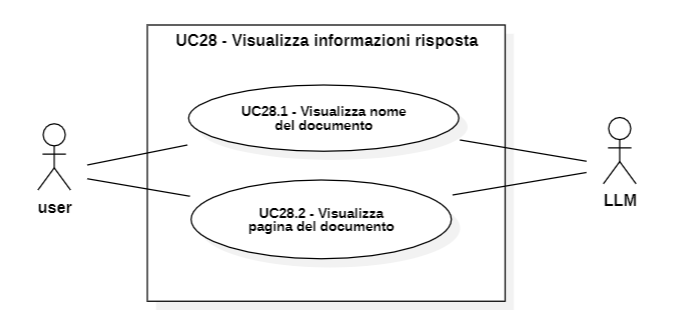
\includegraphics[width=0.9\linewidth]{UC28.1.PNG} 
    \caption{Diagramma UML dei casi d'uso UC-28.1 e UC-28.2}
    \label{fig:UC28.1}
\end{figure}

\subsection{UC-29 Ascolta risposta}
\begin{description}
    \item[Descrizione:] L'utente vuole sentire la lettura della risposta ricevuta.
    \item[Attore primario:] Utente generico.
    \item[Attore secondario:] Modello LLM.
    \item[Pre condizioni:] Il sistema mostra la risposta ad una domanda dell'utente.
    \item[Post condizioni:] Il sistema riproduce la risposta con un audio.
    \item[Scenario:]
    \begin{enumerate}
        \item[]
        \item L’utente pone una domanda al chatbot (\textbf{UC-19}).
        \item Il sistema mostra una risposta alla domanda (\textbf{UC-21}).
        \item L'utente ascolta la risposta ricevuta dal sistema.
    \end{enumerate}
\end{description}

\begin{figure}[H]
    \centering
    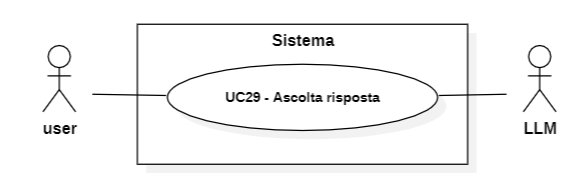
\includegraphics[width=0.9\linewidth]{UC29.png} 
    \caption{Diagramma UML del caso d'uso UC-29}
    \label{fig:UC29}
\end{figure}
